\chapter{膨脹的牛頓宇宙}

\lectureoverview{現代宇宙學始於將宇宙本身視為一個物理系統。從大尺度的各向同性與均勻性出發，我們引入共動網格，並以單一的標度因子\(a(t)\)描述其運動。接著，牛頓球殼定理將引力多體問題化為關於\(a(t)\)的方程。能量守恆將宇宙區分為會再坍縮、處於臨界狀態，以及永遠膨脹的三種情形；物質主導的臨界情形則給出第一個弗里德曼方程，以及\(a(t)\propto t^{2/3}\)這條定律。}

\section{宇宙學何時成為物理學}

宇宙學這門學科源遠流長，但定量宇宙學還很年輕。就此處的目的而言，無須從古希臘談起。較合適的歷史起點，是哈伯在二十世紀第二個四分之一世紀發現宇宙正在膨脹，以及後來人們認出約三開爾文的微波背景是熾熱早期宇宙留下的餘跡。

在測量尚未精確之前，天文學的許多工作必然近似自然史：發現一顆罕見的恆星，分類一個奇特的星系，測量能測量的事物，再編成天體目錄。這些天體當然都是物理系統：它們帶有角動量，含有化學元素，也遵循力學定律。關鍵的轉變，是把\emph{整個宇宙}視為一個物理系統，並以精確到足以接受觀測檢驗的方程來描述它。

這就是本章的主題。我們不只羅列宇宙包含哪些事物，還要探問它的變數、運動與動力學定律。方程並非事後添加的裝飾；它們讓宇宙成為一個物理問題。

從歷史來看，人們是以廣義相對論的語言理解膨脹宇宙。然而，從邏輯上說，最初論證的很大一部分屬於牛頓力學。若有一位十七世紀的物理學家猜對了正確的大尺度運動，他本可以推導出相當不錯的模型。從牛頓力學開始，並不是要取代相對論，而是要揭示那些後來由相對論以幾何方式重新組織的力學內容。

\section{各向同性、均勻性與宇宙學原理}

第一步是觀測。在足夠大的尺度上，宇宙近似\emph{各向同性}：將天空不同區域的情形取平均，並排除銀河系前景的影響後，宇宙在各個方向看起來大致相同。這不表示宇宙完全均勻。近處有恆星的方向，和沒有明顯天體的方向並不相同；物質分布也確實具有結構。各向同性指的是經過平均的大尺度特性。

均勻性則是另一項陳述，意思是經過平均的宇宙在各處都相同。一位身處許多星系之外的觀測者，經過同樣的大尺度平均後，應當會看到大致與我們所見相同類型的宇宙。

作為第一階近似，可以把一個星系簡單視為一個質點。可觀測宇宙大約有
\begin{equation}
N_{\rm gal}\sim 10^{11}
\end{equation}
個星系，每個星系約有\(10^{11}\)顆恆星。因此，恆星總數約為\(10^{22}\)顆。若刻意以每顆恆星有十顆行星作為粗略的數量級估計，便得到\(10^{23}\)顆行星；有趣的是，這接近一莫耳的行星。這項數量估計不屬於動力學的一部分，但能讓我們掌握理想化系統的尺度。

\begin{classroomqa}
\classquestion{可觀測宇宙中大約有多少個星系？}
\lecturerresponse{大約一千億個，也就是\(10^{11}\)。若每個星系約有\(10^{11}\)顆恆星，可見宇宙便約有\(10^{22}\)顆恆星。即使下文的計算會把每個星系視為單一質點，這些數量仍是值得記住的尺度估計。\lecturetimestamp{00:06:08--00:07:05}}
\end{classroomqa}

為什麼我們周圍的各向同性會暗示均勻性？設想一種各向同性但\emph{不}均勻的分布。它的密度必須隨著與我們的距離而變化，同時不隨方向改變；換言之，這種分布會以我們所在的位置為中心，形成同心球殼。一位偏離共同中心的觀測者就不會再看到各向同性。因此有兩種可能：
\begin{enumerate}
\item 我們位於一個特殊中心，宇宙是以此處為中心安排的；或者
\item 大尺度分布近似均勻，因此沒有任何一個被佔據的位置特別突出。
\end{enumerate}
第二種可能較為簡約。若接受各向同性，又不賦予自身特殊的宇宙位置，便會推得均勻性。

\begin{classroomqa}
\classquestion{各向同性但不均勻的分布可能呈現什麼形式？}
\lecturerresponse{它的變化可以只取決於與我們的距離，形成以我們所在位置為中心的球殼狀分布。若觀測者移離該中心，這種分布便不再呈現各向同性。除非我們的位置特殊，各向同性因此指向均勻性。\lecturetimestamp{00:07:06--00:08:54}}
\end{classroomqa}

這項合併假設稱為\emph{宇宙學原理}：在足夠大的尺度上，宇宙在空間中均勻且各向同性。稱它為原理，並不能證明它成立。歷史上，宇宙學家在觀測尚未提供有力依據之前，就採用了這項假設。它之所以站得住腳，靠的是經驗上的成功。

均勻性也不是嚴格成立的。星系會形成星系團與超星系團，而延伸至可見天空很大區域的結構，也早已引發討論。較恰當的說法是，只要平均區域夠大，漲落就會在平均過程中消失---在此處的入門討論中，這個尺度約為數億至十億光年。觀測可以進一步修正這個尺度；所用的方法是持續進行粗粒化，直到局部結構不再主導整體描述。

\begin{classroomqa}
\audiencequestion{宇宙微波背景的均勻性是否支持宇宙學原理？}
\lecturerresponse{是。宇宙學原理提出之時，還沒有充分的觀測依據支持它；但後來的微波背景觀測顯示，原初宇宙極其平滑。星系與星系團是由這種平滑狀態中的微小偏差逐漸形成的，並未抹去支持宇宙大尺度均勻性的證據。\lecturetimestamp{00:10:53--00:11:43}}
\end{classroomqa}

\section{隨星系共動的網格}

選定觀測上的近似之後，就必須選擇變數。有人在課堂上問「表述物理問題的第一步是什麼？」，一種回答是了解變數；傳統的回答則是先把鉛筆削尖。此處的重要變數，是透過妥善選擇座標找出來的。

想像一個帶有標記\(x,y,z\)的三維網格。這些標記不必代表以公尺量度的距離；它們只是座標值。選取適當的網格，使小尺度的特殊運動經過平均後，每個星系都留在固定的網格點上。這些星系便是\emph{共動的}。

如果星系各自隨機移動，這種選擇就毫無用處。但觀測顯示，大尺度上存在一致的運動。相鄰網格單元可以膨脹或收縮，而這種膨脹或收縮在各處都相同。因此，所有物理距離都可以寫成一個共同的時間相依尺度，乘上固定的座標間隔。

對兩個星系\(A\)與\(B\)而言，
\begin{equation}
\begin{aligned}
d_{AB}(t)&=a(t)\,\Delta\chi_{AB},\\
\Delta\chi_{AB}
&=\sqrt{(x_A-x_B)^2+(y_A-y_B)^2+(z_A-z_B)^2}.
\end{aligned}
\label{eq:c01-physical-distance}
\end{equation}
若它們只在\(x\)座標上不同，上式便簡化為
\begin{equation}
d_{AB}(t)=a(t)\,\Delta x_{AB}.
\end{equation}
函數\(a(t)\)稱為\emph{標度因子}。它的絕對歸一化是任意約定：將所有共動座標乘上一個常數，並將\(a\)除以相同常數，不會改變任何物理距離。像\(a(t_2)/a(t_1)\)這樣的比值，以及除以\(a\)的導數，才包含物理資訊。

對方程~\eqref{eq:c01-physical-distance}微分。由於共動間隔固定，
\begin{equation}
v_{AB}=\dot a\sqrt{(\Delta x)^2+(\Delta y)^2+(\Delta z)^2}.
\end{equation}
兩邊除以物理距離，得到
\begin{equation}
\frac{v_{AB}}{d_{AB}}=\frac{\dot a}{a}\equiv H(t),
\label{eq:c01-hubble-parameter}
\end{equation}
也就是
\begin{equation}
\boxed{v_{AB}=H(t)d_{AB}.}
\label{eq:c01-hubble-law}
\end{equation}
這是理想均勻流中的哈伯定律。

「哈伯常數」這個名稱容易造成誤解。在均勻模型的同一宇宙時刻，\(H\)在各處都相同；但\(H(t)\)一般會隨時間改變。空間上處處相同，不代表時間上保持不變。

\begin{classroomqa}
\audiencequestion{把每個距離都寫成共同的\(a(t)\)乘上固定的座標間隔，是否已經假設了哈伯定律？}
\lecturerresponse{這個假設確實受到哈伯觀測的啟發；若沒有星系一致退行的證據，我們不會憑空猜到它。它的作用是將這些觀測整理成一個簡潔的描述：無須為每個星系指定各自的速度，只要描述一個共同膨脹的網格。採用這種描述後，比例關係\(v=Hd\)便可由微分得出。\lecturetimestamp{00:24:20--00:25:33}}
\end{classroomqa}

同一種運動可以用兩種方式描述：星系在空間中彼此遠離；或者星系留在固定的共動位置，而網格---也就是星系之間的物理空間---正在膨脹。在這個階段，兩者只是描述相同數學關係的不同座標說法。廣義相對論會讓「空間膨脹」這種說法格外自然，但只要兩種描述在每個時刻都給出相同的物理間隔，觀測就無法分辨它們。

\section{共動元胞中的質量守恆}

引入引力之前，先記錄質量。考慮一個小的座標元胞，其座標體積為
\begin{equation}
\Delta V_{\rm com}=\Delta x\,\Delta y\,\Delta z.
\end{equation}
但元胞仍須大到足以包含許多星系，以便將局部漲落平均掉。令\(\nu\)表示每單位共動座標體積的質量。元胞中的質量為
\begin{equation}
\Delta M=\nu\,\Delta x\,\Delta y\,\Delta z.
\label{eq:c01-comoving-mass}
\end{equation}
由於元胞隨物質共動，在理想流動中沒有星系穿越其邊界，因此\(\Delta M\)保持不變。

每條物理邊的長度都是相應座標邊長的\(a(t)\)倍。因此，物理體積為
\begin{equation}
\Delta V_{\rm phys}=a^3(t)\,\Delta x\,\Delta y\,\Delta z.
\end{equation}
物理質量密度則為
\begin{equation}
\boxed{\rho(t)=\frac{\Delta M}{\Delta V_{\rm phys}}=\frac{\nu}{a^3(t)}.}
\label{eq:c01-density-dilution}
\end{equation}
膨脹會使無壓物質的密度按\(a^{-3}\)的規律稀釋；收縮則按同一規律使物質聚集。

到目前為止，我們還沒有作任何動力學假設。用到的只有歐幾里得幾何、運動學假設，以及共動元胞中的質量守恆。現在，引力登場了。

\section{現在引入牛頓力學}

有一種看似合理、其實錯誤的圖像：無限且均勻的物質分布應保持靜止，因為一側的引力會被另一側抵消。問題在於，這種非正式的抵消方式，無法為相對加速度建立一致的方程。牛頓球殼定理提供了正確的受力分析方式。

任選一個星系作為原點\(O\)，再考慮一個位於固定共動半徑的星系\(A\)：
\begin{equation}
R=\sqrt{x^2+y^2+z^2}.
\end{equation}
其物理半徑、徑向速度與徑向加速度分別為
\begin{equation}
d=aR,
\qquad
\dot d=\dot a R,
\qquad
\ddot d=\ddot a R.
\label{eq:c01-radial-kinematics}
\end{equation}

\begin{figure}[ht]
\centering
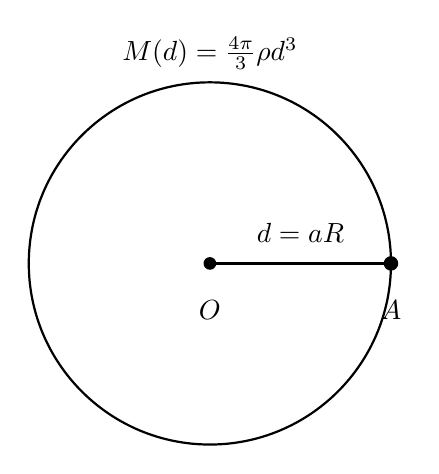
\begin{tikzpicture}[scale=1.15]
\draw[thick] (0,0) circle (2);
\fill (0,0) circle (0.07);
\fill (2,0) circle (0.08);
\draw[thick] (0,0) -- (2,0);
\draw (1,0.12) node[above] {\(d=aR\)};
\draw (0,-0.3) node[below] {\(O\)};
\draw (2,-0.3) node[below] {\(A\)};
\draw (0,2.32) node {\(M(d)=\frac{4\pi}{3}\rho d^3\)};
\end{tikzpicture}
\caption{牛頓力學的化簡。計算星系\(A\)的加速度時，外部球殼的引力相互抵消，而半徑\(d\)以內的質量，對它的作用就如同全部集中在\(O\)。}
\label{fig:c01-newton-sphere}
\end{figure}

對球對稱的質量分布而言，球面\(A\)之外的物質所產生的合力為零。球面內的物質，其作用等同於集中在球心。包圍的質量為
\begin{equation}
M(d)=\frac{4\pi}{3}\rho d^3.
\label{eq:c01-enclosed-mass}
\end{equation}
接著，牛頓平方反比定律給出星系\(A\)的加速度：
\begin{equation}
\ddot d=-\frac{GM(d)}{d^2}.
\end{equation}
利用方程~\eqref{eq:c01-radial-kinematics}，
\begin{align}
\ddot a R
&=-\frac{G}{d^2}\left(\frac{4\pi}{3}\rho d^3\right) \\
&=-\frac{4\pi G}{3}\rho d \\
&=-\frac{4\pi G}{3}\rho aR.
\end{align}
共動半徑相消後，得到
\begin{equation}
\boxed{\frac{\ddot a}{a}=-\frac{4\pi G}{3}\rho.}
\label{eq:c01-acceleration}
\end{equation}
這個相消結果檢驗了模型是否自洽。所有共動星系，無論\(R\)取何值，都遵循同一個關於同一標度因子的方程。

將方程~\eqref{eq:c01-density-dilution}代入，可得以下兩種等價形式：
\begin{equation}
\frac{\ddot a}{a}=-\frac{4\pi G\nu}{3a^3},
\qquad
\ddot a=-\frac{4\pi G\nu}{3a^2}.
\label{eq:c01-acceleration-nu}
\end{equation}
第一種形式顯示的是分數加速度；第二種則將\(\ddot a\)單獨寫出。把\(a\)留在等號左側只是記號上的慣例，不會改變物理內容。

\begin{classroomqa}
\audiencequestion{原點是任意選的，但計算中的每個力都指向它。為什麼改選另一個原點，仍會得到同一個宇宙？}
\lecturerresponse{這個方程描述的是相對運動。以任何其他星系為中心重做計算，都會得到相同方程，因為均勻性使包圍的質量只取決於物理半徑。若轉換到附著於另一星系的加速參考系，卻仍沿用相對於第一個原點定義的力，就必須一併計入相應的慣性力。選擇一個中心靜止參考系，只是省下這筆額外的計算。真正不變的結果是方程~\eqref{eq:c01-acceleration}，而不是某個特殊中心。\lecturetimestamp{00:43:56--00:46:58}}
\end{classroomqa}

\begin{classroomqa}
\audiencequestion{如果共動質量密度\(\nu\)隨位置改變，這個結果還成立嗎？}
\lecturerresponse{以單一函數描述的形式便不再成立。能如此簡潔地相消，仰賴\(M\propto d^3\)在各處都具有相同的比例關係。若\(\nu\)在平均尺度內有顯著變化，不同區域就需要各自的局部動力學，單一的均勻標度因子也就無法再描述整個系統。均勻性在此扮演關鍵角色。\lecturetimestamp{00:47:05--00:47:51}}
\end{classroomqa}

\begin{classroomqa}
\audiencequestion{為什麼寫成\(\ddot a/a\)，而不把因子\(a\)移到等號右邊？}
\lecturerresponse{兩種寫法都正確。宇宙學慣例上採用分數加速度\(\ddot a/a\)，部分原因是它可以直接與分數膨脹率\(H=\dot a/a\)比較。等式兩邊乘以\(a\)，就會得到完全相同的微分方程。\lecturetimestamp{00:50:36--00:51:29}}
\end{classroomqa}

方程~\eqref{eq:c01-acceleration}立即排除了充滿普通物質的靜態均勻牛頓宇宙。若標度因子靜止，便有\(\ddot a=0\)；但只要密度為正，方程右側就是負值。這\emph{尚未}告訴我們宇宙正在膨脹還是收縮，只能告訴我們加速度的符號。

\section{負加速度不等於收縮}

速度與加速度的區別看似基本，卻至關重要。在德國高速公路上向前行駛的法拉利，即使在煞車減速，加速度為負，速度仍可以是正的。同樣，宇宙也可以滿足
\begin{equation}
\dot a>0,
\qquad
\ddot a<0:
\end{equation}
也就是仍在膨脹，只是膨脹速度正在減慢。

要判斷運動是否最終反向，可以把宇宙學問題與在地球引力場中沿徑向運動的試驗粒子相比。現在以\(x\)表示粒子到中心質量\(M\)的物理距離；它與前面使用的共動座標無關。牛頓方程為
\begin{equation}
\ddot x=-\frac{GM}{x^2}.
\label{eq:c01-particle-force}
\end{equation}
加速度始終朝內。即使如此，被向外拋出的粒子仍可能繼續向外運動很久，甚至永遠不回頭。已經向內運動的粒子，其速度則會愈來愈負。僅憑力定律無法判定粒子會如何運動；還需要知道初始條件。

\begin{classroomqa}
\audiencequestion{\(\ddot a<0\)是否表示宇宙正在收縮？}
\lecturerresponse{不是。收縮表示\(\dot a<0\)。\(\ddot a\)為負，只表示\(\dot a\)隨時間減小。如果\(\dot a\)一開始為正，引力就會讓膨脹減慢；它是否會降至零，取決於初始膨脹速度，正如向外運動的拋射物能否逃逸，取決於其速度低於還是高於逃逸速度。\lecturetimestamp{00:51:30--00:56:18}}
\end{classroomqa}

\begin{figure}[ht]
\centering
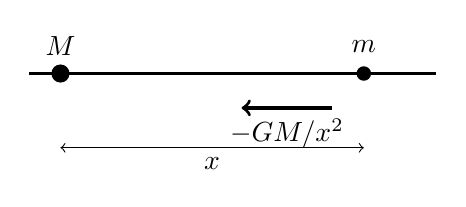
\begin{tikzpicture}[scale=1.15]
\fill (0,0) circle (0.1);
\draw (0,0.3) node {\(M\)};
\draw[thick] (-0.35,0) -- (4.15,0);
\fill (3.35,0) circle (0.08);
\draw (3.35,0.3) node {\(m\)};
\draw[->,very thick] (3.0,-0.38) -- (2.0,-0.38)
  node[midway,below] {\(-GM/x^2\)};
\draw[<->] (0,-0.82) -- (3.35,-0.82)
  node[midway,below] {\(x\)};
\end{tikzpicture}
\caption{這個徑向單粒子問題，說明了加速度的符號與運動方向及最終結果是不同的概念。}
\label{fig:c01-particle-sketch}
\end{figure}

能量守恆讓各種可能性一目了然。守恆的力學能為
\begin{equation}
E=\frac12 m\dot x^{\,2}-\frac{GMm}{x}.
\label{eq:c01-particle-energy}
\end{equation}
勢能與\(1/x\)成正比，而非與\(1/x^2\)成正比；對\(-GMm/x\)微分後，會得到平方反比力。

\begin{figure}[ht]
\centering
\includegraphics[width=0.82\textwidth]{lecture_01_figure_02.png}
\caption{能量論證開始時的板書：一個正在運動的試驗質量及其動能項，接著才要補上引力勢能。}
\lectureframe{00:58:57}
\end{figure}

若\(E<0\)，向外運動的粒子無法到達無窮遠；在那裡，勢能趨近於零，而動能不可能為負。因此粒子必定會在有限的\(x\)處停下，然後返回。若\(E>0\)，粒子就不可能停下：在轉折點，動能為零，剩餘的勢能則為負，這與正的\(E\)守恆相矛盾。兩者的分界為
\begin{equation}
E=0,
\end{equation}
由此定義逃逸速度：
\begin{equation}
\frac12 m v_{\rm esc}^2-\frac{GMm}{x}=0,
\qquad
\boxed{v_{\rm esc}^2=\frac{2GM}{x}.}
\label{eq:c01-escape-velocity}
\end{equation}

\begin{figure}[ht]
\centering
\includegraphics[width=0.88\textwidth]{lecture_01_figure_03.png}
\caption{零能量的分界正在板書上逐漸成形。先前的宇宙學加速度方程仍框在左側，右側則開始推導徑向逃逸問題。}
\lectureframe{01:01:37}
\end{figure}

粒子恰好以逃逸速度運動時，會持續減速。只有在\(x\to\infty\)時，它的速率才趨近於零；它不會在任何有限距離處抵達轉折點。這個邊界情形將是最簡單的宇宙學模型。

\section{宇宙學能量方程}

回到一個位於固定共動半徑\(R\)處的星系。根據球殼定理，它的徑向運動等同於一個粒子在點質量外側的運動，而該點質量等於共動球所包圍的質量。

\begin{figure}[ht]
\centering
\includegraphics[width=0.82\textwidth]{lecture_01_figure_04.png}
\caption{將單粒子的能量論證帶回宇宙學時所用的平方反比力與徑向粒子示意圖。}
\lectureframe{01:04:14}
\end{figure}

物理球面擴大時，球內的質量並不會增加。球面隨物質共動，因此始終包圍相同的星系：
\begin{align}
M
&=\frac{4\pi}{3}\rho(aR)^3 \\
&=\frac{4\pi}{3}\frac{\nu}{a^3}a^3R^3 \\
&=\frac{4\pi}{3}\nu R^3.
\label{eq:c01-fixed-enclosed-mass}
\end{align}
第一個式子看似隨時間變化，是因為尚未將密度稀釋納入考慮；\(a^3\)中的因子會相消。

\begin{classroomqa}
\audiencequestion{球面擴大時，包圍的質量會增加嗎？}
\lecturerresponse{不會。物理半徑雖然增大，共動邊界卻隨星系移動。在理想的均勻流動中，沒有物質穿越這道邊界；方程~\eqref{eq:c01-fixed-enclosed-mass}明確顯示了各項如何相消。\lecturetimestamp{01:04:37--01:05:20}}
\end{classroomqa}

星系的物理速度為\(\dot d=\dot a R\)，與所選原點的距離為\(d=aR\)。因此，其守恆的牛頓力學能量為
\begin{equation}
\boxed{
E=\frac12 m\dot a^{\,2}R^2-\frac{GMm}{aR}.
}
\label{eq:c01-cosmological-energy}
\end{equation}

\begin{figure}[ht]
\centering
\includegraphics[width=0.82\textwidth]{lecture_01_figure_05.png}
\caption{板書上的宇宙學動能項與勢能項。方程~\eqref{eq:c01-cosmological-energy}中完整的分母\(aR\)，來自物理半徑及其相關推導。}
\lectureframe{01:06:12}
\end{figure}

粒子能量的三種情形，對應宇宙學的三種情形：
\begin{description}[style=nextline]
\item[\(E<0\)：]初始膨脹速度低於逃逸速度；\(a(t)\)到達最大值後，宇宙再度坍縮。
\item[\(E=0\)：]宇宙正好處於臨界狀態；膨脹永遠持續減慢，速度只會漸近地趨近於零。
\item[\(E>0\)：]初始膨脹速度高於逃逸速度；在牛頓模型中，宇宙將永遠膨脹，且其漸近退行速度不為零。
\end{description}

我們先考慮邊界情形\(E=0\)。令方程~\eqref{eq:c01-cosmological-energy}等於零，消去\(m\)，再除以\(a^2R^2/2\)，得到
\begin{align}
\frac12\dot a^{\,2}R^2&=\frac{GM}{aR}, \\
\left(\frac{\dot a}{a}\right)^2&=\frac{2GM}{a^3R^3}.
\label{eq:c01-energy-intermediate}
\end{align}
又因為
\begin{equation}
\rho=\frac{M}{(4\pi/3)a^3R^3},
\end{equation}
方程~\eqref{eq:c01-energy-intermediate}便成為
\begin{equation}
\boxed{
H^2=\left(\frac{\dot a}{a}\right)^2=\frac{8\pi G}{3}\rho.
}
\label{eq:c01-first-friedmann}
\end{equation}
這就是空間平坦、只有物質且宇宙學常數為零的宇宙之第一個弗里德曼方程；此處是由牛頓力學中的能量守恆推導而得。

\begin{classroomqa}
\classquestion{粒子恰好以逃逸速度發射時，會發生什麼事？}
\lecturerresponse{粒子會減速，卻永遠不會反向；只有到達無窮遠時，速度才會趨近於零。零能量宇宙也有相同的行為：\(H\)逐漸減小，但\(\dot a\)仍保持為正，不會在有限時間內停止膨脹並反轉。\lecturetimestamp{01:10:45--01:12:10}}
\end{classroomqa}

因子\(4\pi/3\)與\(8\pi G/3\)並非任意添加的裝飾。\(4\pi/3\)代表球體積，而因子二來自動能。在廣義相對論中，同一個\(8\pi G\)也出現在愛因斯坦場方程裡；其時間—時間分量會導出相對論的弗里德曼方程。這種一致性並非偶然，不過目前的推導尚未納入壓力、作為幾何性質的空間曲率，或宇宙學常數。

\section{物質主導的臨界解}

將密度定律\(\rho=\nu/a^3\)代入方程~\eqref{eq:c01-first-friedmann}：
\begin{equation}
\left(\frac{\dot a}{a}\right)^2=\frac{8\pi G\nu}{3a^3}.
\label{eq:c01-matter-friedmann}
\end{equation}
常數\(\nu\)取決於共動座標的任意歸一化。為了凸顯時間相依性，定義
\begin{equation}
K\equiv\frac{8\pi G\nu}{3}>0.
\end{equation}
於是
\begin{equation}
\dot a^{\,2}=\frac{K}{a}.
\label{eq:c01-normalized-friedmann}
\end{equation}

\begin{figure}[ht]
\centering
\includegraphics[width=0.76\textwidth]{lecture_01_figure_06.png}
\caption{板書上的物質主導弗里德曼尺度關係：先寫出含常數的形式，再凸顯標度因子的主要反比冪次。}
\lectureframe{01:14:44}
\end{figure}

方程~\eqref{eq:c01-normalized-friedmann}右側對任何有限且為正的\(a\)都為正。若要發生轉折，就必須有\(\dot a=0\)；因此，臨界宇宙永遠不會轉折。它的膨脹愈來愈慢，卻永遠不會慢到停下來。

現在來解這個方程。可以直接分離變數：
\begin{equation}
a^{1/2}\,da=\sqrt{K}\,dt,
\end{equation}
也可以如課堂推導所示，試設為冪律形式：
\begin{equation}
a(t)=Ct^p.
\label{eq:c01-power-trial}
\end{equation}
於是
\begin{equation}
\frac{\dot a}{a}=\frac{p}{t},
\qquad
\frac{K}{a^3}=\frac{K}{C^3t^{3p}}.
\end{equation}
代入方程~\eqref{eq:c01-matter-friedmann}，得到
\begin{equation}
\frac{p^2}{t^2}=\frac{K}{C^3t^{3p}}.
\end{equation}
比較冪次與係數，可得
\begin{equation}
3p=2,
\qquad
C^3=\frac{K}{p^2}=\frac{9K}{4}.
\end{equation}
因此
\begin{equation}
\boxed{
a(t)=\left(\frac{3\sqrt K}{2}t\right)^{2/3}\propto t^{2/3}.
}
\label{eq:c01-two-thirds}
\end{equation}
時間原點的可加常數選為使\(t=0\)時\(a=0\)。更一般地，可將\(t\)換成\(t-t_0\)。

標度因子會持續增長，而
\begin{equation}
\dot a\propto t^{-1/3}\longrightarrow0,
\qquad
H=\frac{2}{3t}\longrightarrow0.
\label{eq:c01-asymptotic-slope}
\end{equation}
其曲線始終遞增且向下凹。由於\(a(t)\)本身沒有上界，曲線不會趨近於水平線，但斜率會趨近於零。

\begin{classroomqa}
\audiencequestion{\(t^{2/3}\)這個結果是不是只因為試設的形式恰好奏效？換一種試設，會不會得到另一個零能量解？}
\lecturerresponse{這個試設找出的是唯一解，而不只是其中一種可能性。對膨脹分支的一階方程\(\dot a=\sqrt{K/a}\)積分後，除歸一化與時間原點的選擇外，唯一得到\(a\propto(t-t_0)^{2/3}\)。總能量不同，微分方程也不同，因此宇宙的演化歷史也不同。\lecturetimestamp{01:27:07--01:27:43}}
\end{classroomqa}

\begin{classroomqa}
\audiencequestion{臨界曲線最後會變成水平線嗎？}
\lecturerresponse{曲線斜率會趨近於零：\(\dot a\propto t^{-1/3}\)。然而在任何有限時刻，斜率都仍為正，因此標度因子會繼續增長而不受限制。宇宙漸近地趨近靜止，卻永遠不會真正靜止。\lecturetimestamp{01:27:48--01:28:57}}
\end{classroomqa}

這個簡單的結果在歷史上頗耐人尋味。牛頓具備推導所需的力學與球殼定理，也思考過無限引力宇宙相關的問題，卻沒有建立膨脹宇宙模型。課堂討論提出一項歷史推測：對宇宙歷史的哲學與神學信念，或許影響了牛頓認為哪些問題值得探究。這項推測與數學推導無關；數學上的重點僅在於，推導所需的牛頓力學工具當時已經存在。

\begin{classroomqa}
\audiencequestion{這個牛頓力學模型是否假設宇宙是無限的？}
\lecturerresponse{它假設牛頓空間為歐幾里得空間且在空間上平坦。在通常的牛頓模型中，這個空間向各處無限延伸，因此模型在空間上是無限的，儘管共動星系間的距離會隨時間改變。彎曲的有限空間幾何，則屬於相對論的處理範疇。\lecturetimestamp{01:22:12--01:22:55}}
\end{classroomqa}

\section{超越零能量模型}

零能量情形是刻意採用的簡化，並非唯一的牛頓宇宙。在方程~\eqref{eq:c01-cosmological-energy}中保留\(E\neq0\)，可得
\begin{equation}
\left(\frac{\dot a}{a}\right)^2
=\frac{8\pi G}{3}\rho+\frac{2E}{mR^2a^2}.
\label{eq:c01-nonzero-energy}
\end{equation}
均勻性要求組合\(2E/(mR^2)\)對每個代表性的共動球都相同。將它記為常數\(C_E\)，則
\begin{equation}
H^2=\frac{8\pi G}{3}\rho+\frac{C_E}{a^2}.
\end{equation}
\(C_E\)為正，代表能量高於逃逸能量；\(C_E\)為負，則容許宇宙轉折。用相對論的記號表示時，這個能量項會以空間曲率重新詮釋；相關連結留待後文討論。

在物質主導期間，這三種僅由物質構成的演化歷程，加速度都為負：
\begin{equation}
\ddot a=-\frac{4\pi G}{3}\rho a<0.
\end{equation}
再坍縮曲線先上升，達到\(\dot a=0\)，再下降。臨界曲線永遠上升，且斜率趨近零，其形式為\(t^{2/3}\)。正能量曲線也永遠上升，並漸近於線性成長。課堂上曾先畫出這些情形的草圖，之後又加以修正；最後確立的結論是，三者都呈凹向下的形狀，至於第一幅草圖的其他細節則不盡正確。

觀測到的宇宙還呈現出另一種行為。早期物質主導的膨脹可由一條減速曲線很好地近似，但到了晚期，曲線會向上彎：
\begin{equation}
\ddot a>0.
\end{equation}
普通的無壓物質無法在方程~\eqref{eq:c01-acceleration}中產生這種加速度。因此，必須加入額外項。在最簡單的現代模型中，這一項是宇宙學常數；更一般地說，它稱為暗能量。本章刻意先省略這一項，以便清楚理解牛頓物質動力學。

\begin{classroomqa}
\audiencequestion{弗里德曼方程中的\(8\pi G\)，是否就是愛因斯坦場方程中出現的同一個因子？我們有沒有納入宇宙學常數？}
\lecturerresponse{廣義相對論中也會出現相同的引力歸一化因子，而場方程的時間－時間分量會重現相對論的弗里德曼方程。這裡的模型沒有納入宇宙學常數。這是物質主導的宇宙；省略的宇宙學常數項，正是能夠解釋晚期加速的那類項。\lecturetimestamp{01:30:15--01:31:06}}
\end{classroomqa}

\section{平均流與局部偏離}

均勻膨脹是一種粗粒化描述。這並不表示每個物體都會遠離所有鄰近物體。受引力束縛或以其他方式束縛的系統，可以脫離哈伯流。例如，銀河系和仙女座星系彼此接近，而非遵循大尺度的退行定律。

單一星系的速度相對於哈伯流的偏離，稱為該星系的\emph{本動速度}。這是技術用語，並非對星系的評價。隨著平均所涵蓋的距離和體積增大，哈伯定律會成為更好的近似。在受束縛星系、星系團或局部過密區域的尺度上，局部作用力可能主導背景膨脹。

\begin{classroomqa}
\audiencequestion{即使宇宙整體在膨脹，某些區域也可能收縮嗎？}
\lecturerresponse{當然可能。束縛系統和密度足夠高的漲落，不必跟隨平均膨脹。銀河系--仙女座星系系統就是一個熟悉的例子。宇宙學計算會對足夠大的體積取平均，使這些本動運動和局部密度漲落不致占主導；所得的\(a(t)\)描述的是背景演化，而非每一對物體的情形。\lecturetimestamp{01:31:00--01:34:13}}
\end{classroomqa}

這可以用普通氣體來類比。說一個房間裡的空氣是均勻的，並不表示分子沒有漲落，也不表示密度沒有局部變化；這只表示在足夠大的區域上取平均，結果會趨於穩定。宇宙均勻性在邏輯上也是如此，只是涉及的尺度大得多。一個形成時密度略高於平均值的區域，可能具有足夠的自引力來抵抗膨脹，最終坍縮成束縛結構。

\begin{classroomqa}
\audiencequestion{觀測能否判定星系是在空間中運動，還是膨脹的空間使它們彼此遠離？}
\lecturerresponse{若兩種描述都為每一對星系指定相同的距離\(d_{AB}(t)\)，就無法判定。一種描述把星系視為在看似固定的座標背景上運動；在共動描述中，星系的位置固定不變，距離的變化則由尺度因子承載。兩種描述在數學上等價。廣義相對論使第二種說法更為自然，但就這項比較而言，它並未帶來另一個可觀測量。\lecturetimestamp{01:34:14--01:34:59}}
\end{classroomqa}

\begin{classroomqa}
\audiencequestion{除了 Ia 型超新星的亮度之外，是否還有宇宙加速膨脹的獨立證據？}
\lecturerresponse{有。這項推論來自多種觀測彼此交織的證據，尤其是超新星測量結果與宇宙微波背景觀測結果相互吻合。沒有任何單一資料足以支撐整個結論；關鍵在於不同宇宙學測量彼此一致。\lecturetimestamp{01:35:00--01:35:38}}
\end{classroomqa}

\section{已確立的結論}

論證依照嚴謹的順序逐步展開：
\begin{enumerate}
\item 大尺度各向同性，加上排除宇宙具有特權中心，促使我們採用均勻性假設。
\item 均勻性使我們得以建立共動網格，並以單一尺度因子\(a(t)\)描述其膨脹。
\item 對物理距離微分，可得哈伯定律：
  \[
  H=\frac{\dot a}{a},
  \qquad
  v=Hd.
  \]
\item 共動體積元中的質量守恆給出：
  \[
  \rho=\frac{\nu}{a^3}.
  \]
\item 牛頓殼層定理給出加速度方程：
  \[
  \frac{\ddot a}{a}=-\frac{4\pi G}{3}\rho.
  \]
\item 守恆能量將膨脹分為再坍縮、臨界和不受束縛三種情形。
\item 總能量為零時，
  \[
  H^2=\frac{8\pi G}{3}\rho,
  \qquad
  a(t)\propto t^{2/3}.
  \]
\end{enumerate}

這是一個完整的牛頓物質主導模型，但還不足以完整描述我們的宇宙。它呈現了早期減速膨脹的物理脈絡，說明為何充滿物質的均勻宇宙不可能維持靜止，並指出位於逃逸臨界點的膨脹情形。非零能量、相對論的空間幾何、壓力、輻射，以及造成晚期加速的項，仍有待納入。